\documentclass[tikz,border=0pt]{standalone}
\usepackage{tgbonum}

\usepackage{amsmath}
\definecolor{bgr}{RGB}{189, 90, 107}
\usepackage{pgf}
\usepackage{tikz}
\usetikzlibrary{arrows, automata, backgrounds}
\usepackage[latin1]{inputenc}
\begin{document}

{\fontfamily{qbk}\selectfont
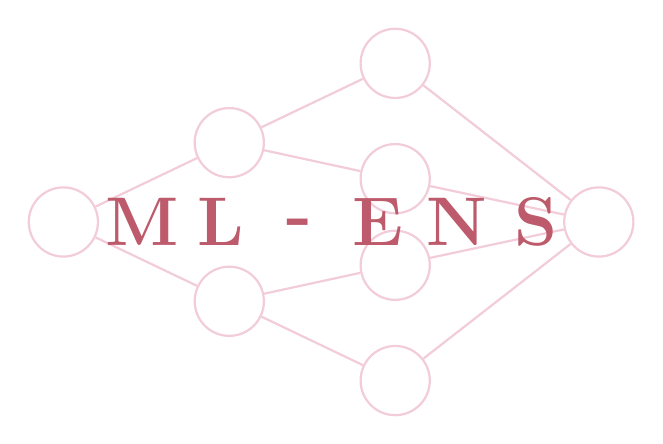
\begin{tikzpicture}[-, node distance=1.cm, thick, inner sep=0pt]





  \node[state, draw=purple!20]  (X)  {};
  \node[state, draw=purple!20]  (X_1) [above right of=X, xshift=1.4cm, yshift=0.3cm]  {};
  \node[state, draw=purple!20]  (X_2) [below right of=X, xshift=1.4cm, yshift=-0.3cm] {};
  \node[state, draw=purple!20]  (P_1) [above right of=X_1, xshift=1.4cm, yshift=0.3cm] {};
  \node[state, draw=purple!20]  (P_2) [below right of=X_1, xshift=1.4cm, yshift=0.25cm] {};
  \node[state, draw=purple!20]  (P_3) [above right of=X_2, xshift=1.4cm, yshift=-0.25cm] {};
  \node[state, draw=purple!20]  (P_4) [below right of=X_2, xshift=1.4cm, yshift=-0.3cm] {};
  \node[state, draw=purple!20]  (Y)   [right of=X, node distance=6.8cm]{};


  \path (X) edge [purple!20]  (X_1)
        (X) edge [purple!20]  (X_2)
        (X_1) edge [purple!20]  (P_1)
        (X_1) edge [purple!20]  (P_2)
        (X_2) edge [purple!20]  (P_3)
        (X_2) edge [purple!20]  (P_4)
        (P_1) edge [purple!20]  (Y)
        (P_2) edge [purple!20]  (Y)
        (P_3) edge [purple!20]  (Y)
        (P_4) edge [purple!20]  (Y)
        ;
\node[state, draw=none] at (1, 0) (M) [] {\textcolor{bgr}{\Huge \textsf{\bf{M}}}};
\node[state, draw=none] at (2, 0) (M) [] {\textcolor{bgr}{\Huge \textsf{\bf{L}}}};
\node[state, draw=none] at (3, 0) (M) [] {\textcolor{bgr}{\Huge \textsf{\bf{-}}}};
\node[state, draw=none] at (4, 0) (M) [] {\textcolor{bgr}{\Huge \textsf{\bf{E}}}};
\node[state, draw=none] at (5, 0) (M) [] {\textcolor{bgr}{\Huge \textsf{\bf{N}}}};
\node[state, draw=none] at (6, 0) (M) [] {\textcolor{bgr}{\Huge \textsf{\bf{S}}}};



\end{tikzpicture}
}
\end{document}
